\subsection{Model fitting}
\label{subsec:fitting}
We employed a Markov Chain Monte Carlo (MCMC) script to fit the coefficients of a polynomial model for $r(\mathcal{M}_c)$. The MCMC uses the smoothing prior as defined in \S\ref{subsec:likelihood}. We performed a least squares fit first in order to obtain the initial guess for the coefficients of the model.

The model we used is a polynomial of degree 9. Because of the smoothing function, using higher order does not change the shape of the fit in a significant way. The MCMC best fit can be seen in Figure \ref{fig:line_MCMC}. The MCMC walkers and triangle plot are in Figures \ref{fig:MCMC_time} and \ref{fig:MCMC_triangle}.

Best fit model is:
\begin{equation}
\begin{split}
\label{MCMC_best_fit}
r(\mathcal{M}_c) = \sum_{k = 0}^{9}\alpha_k(\log\mathcal{M}_c)^k
\end{split}
\end{equation}

Where the coefficients, $\alpha_k$, are listed in Table \ref{table:coefficients}.

\begin{table}[ht]
\centering
\caption{Coefficients from the MCMC fit.}
\label{table:coefficients}

\begin{tabular}{l|r}
  k & $\alpha_k$ \\
  \hline
  \hline
  0 & \num{-1.903e-06} \\
  1 & \num{+1.842e-05} \\
  2 & \num{+9.999e-01} \\
  3 & \num{+1.748e-04} \\
  4 & \num{-2.441e-04} \\
  5 & \num{+2.122e-04} \\
  6 & \num{-1.130e-04} \\
  7 & \num{+3.470e-05} \\
  8 & \num{-5.416e-06} \\
  9 & \num{+3.470e-07} \\
\end{tabular}
\end{table}

\begin{figure*}[ht]
  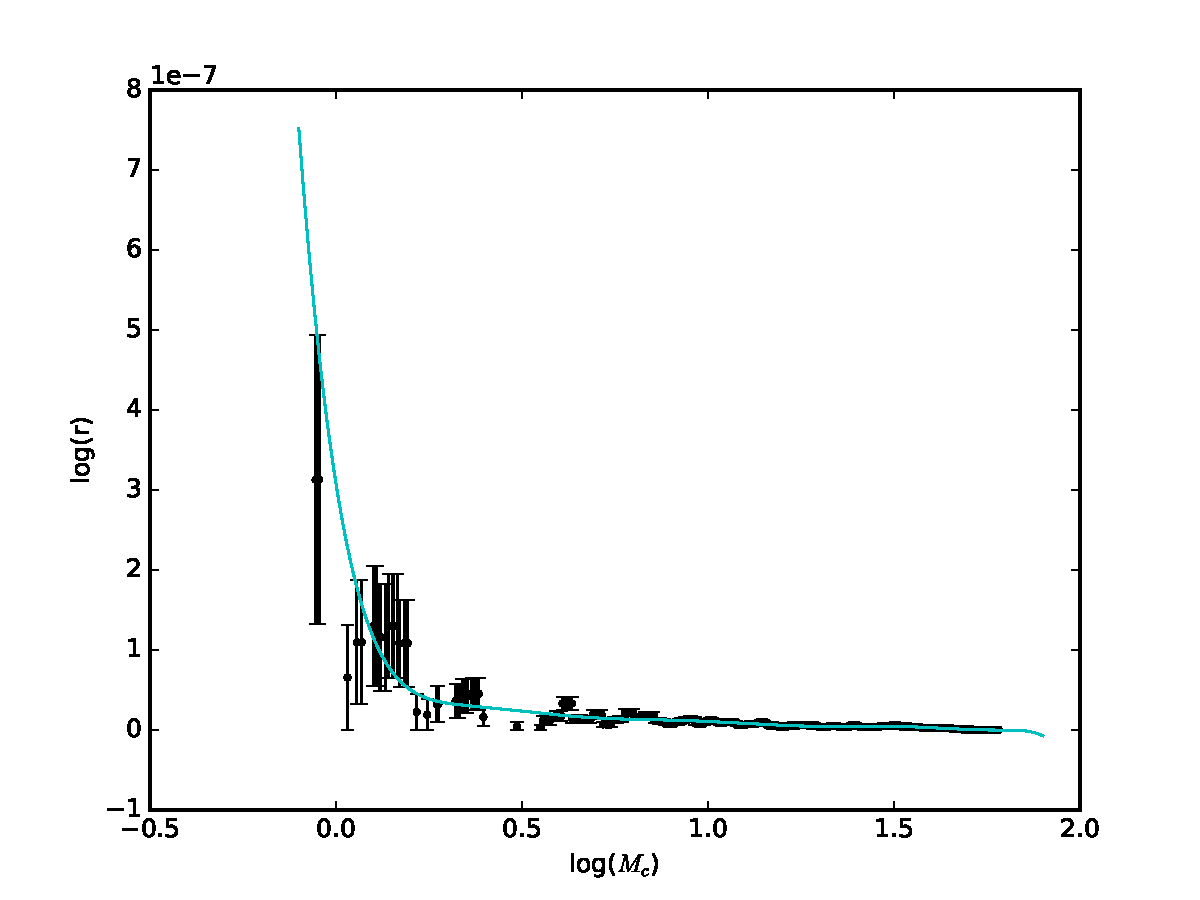
\includegraphics[width=\textwidth]{img/line-MCMC.pdf}
  \caption{The cyan line is an example of a fit from MCMC.}
  \label{fig:line_MCMC}
\end{figure*}

\begin{figure*}[ht]
  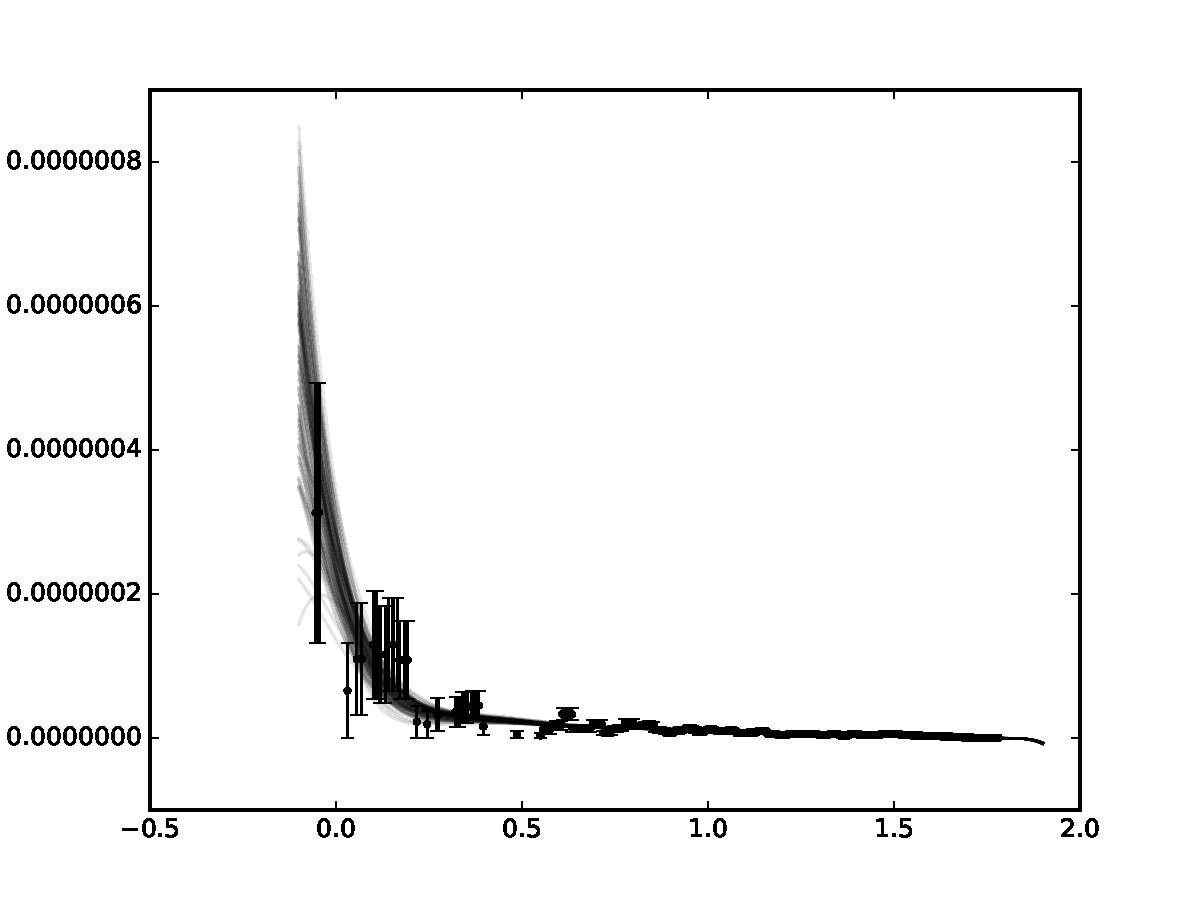
\includegraphics[width=\textwidth]{img/line-mcmc_err.pdf}
  \caption{2000 randomly chosen fits from the MCMC.}
  \label{fig:line_MCMC_err}
\end{figure*}

\begin{figure*}[ht]
  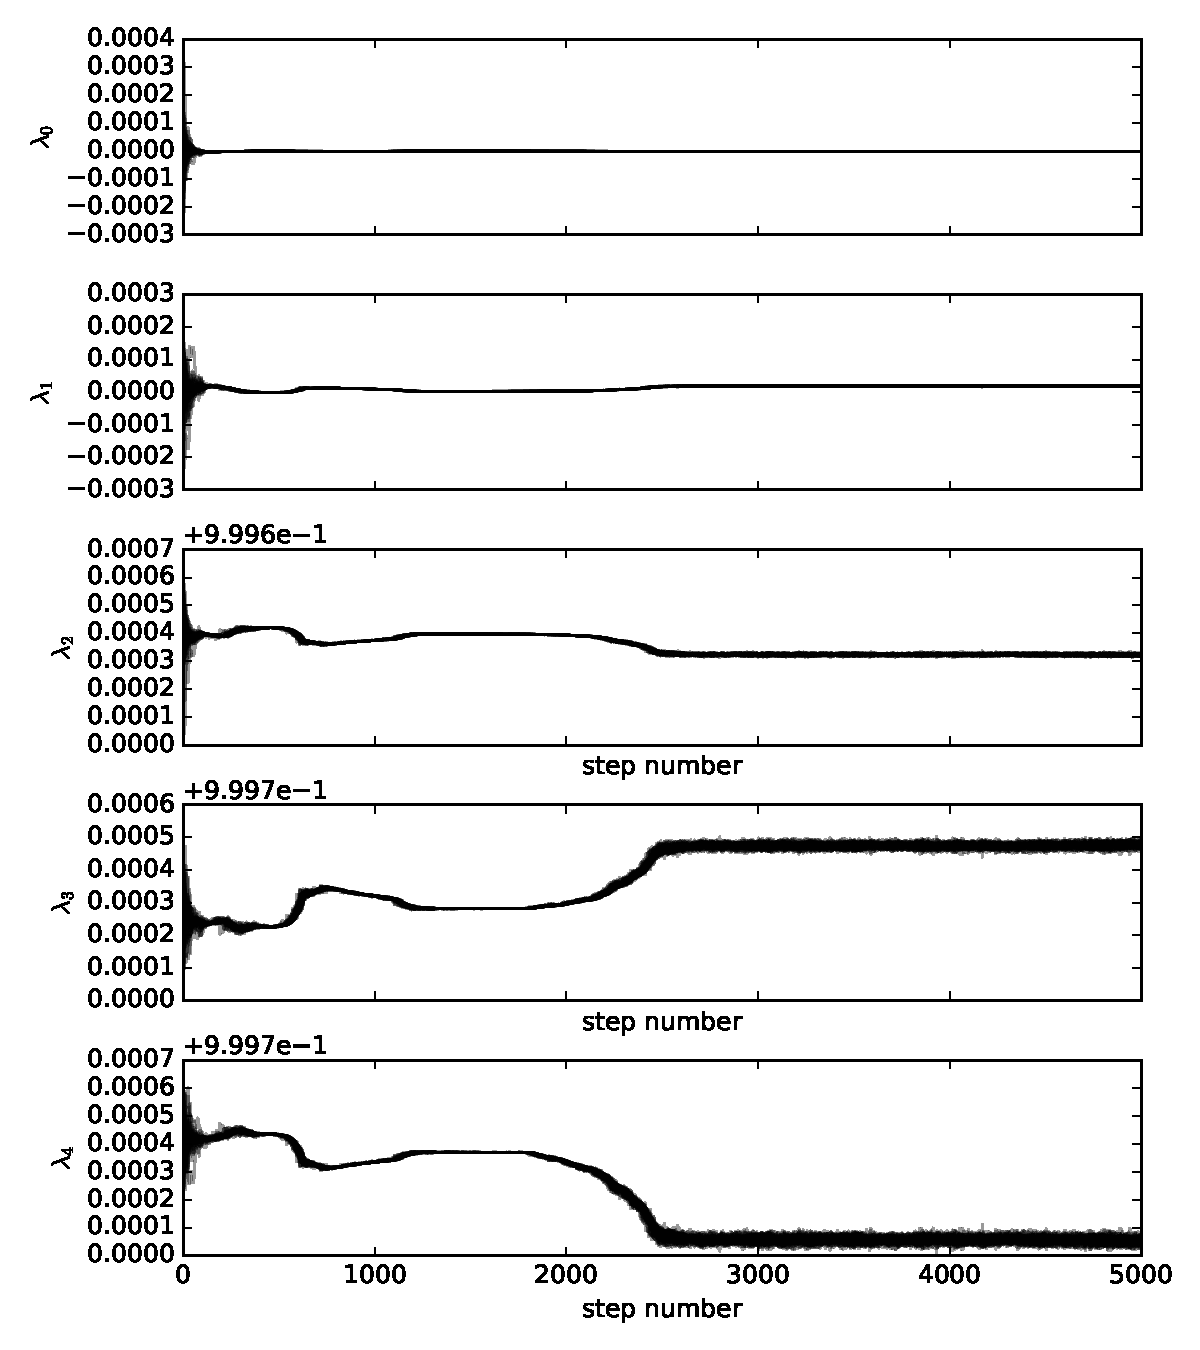
\includegraphics[width=\textwidth]{img/line-time-1.pdf}
  \caption{Visualization of MCMC worker locations over the large number of iterations performed for coefficients $\lambda_0 $ to $\lambda_4$. }
  \label{fig:MCMC_time}
\end{figure*}

\begin{figure*}[ht]
  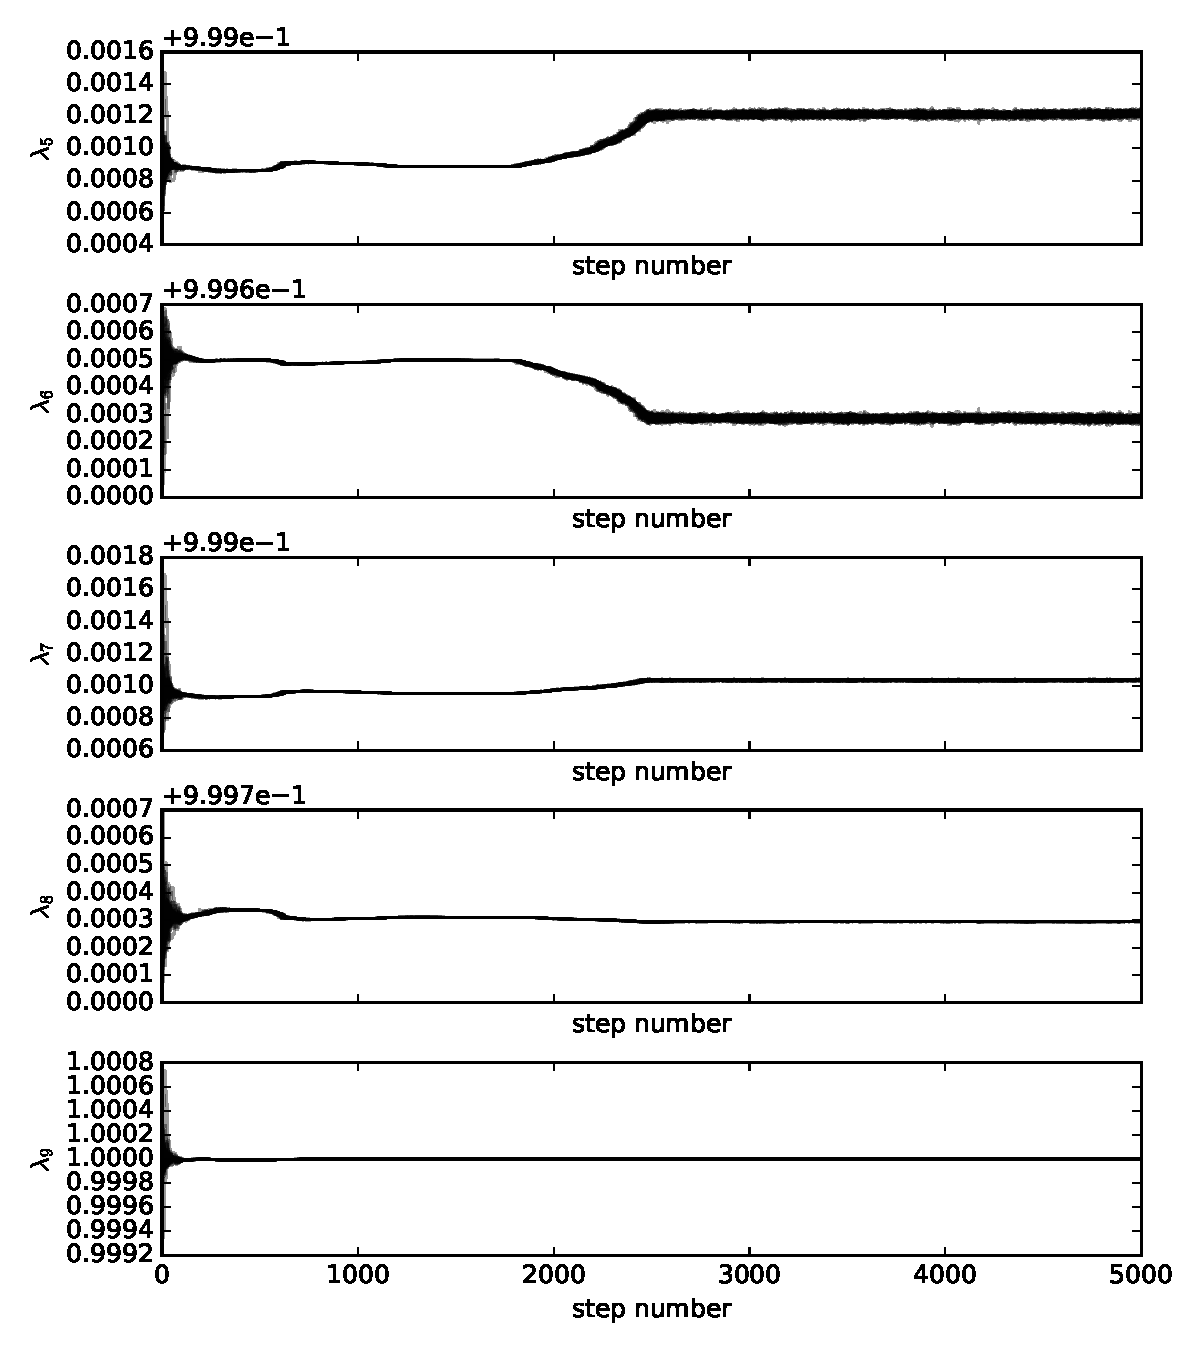
\includegraphics[width=\textwidth]{img/line-time-2.pdf}
  \caption{Visualization of MCMC worker locations over the large number of iterations performed for coefficients $\lambda_5$ to $\lambda_9$.}
  \label{fig:MCMC_time}
\end{figure*}

\begin{figure*}[ht]
  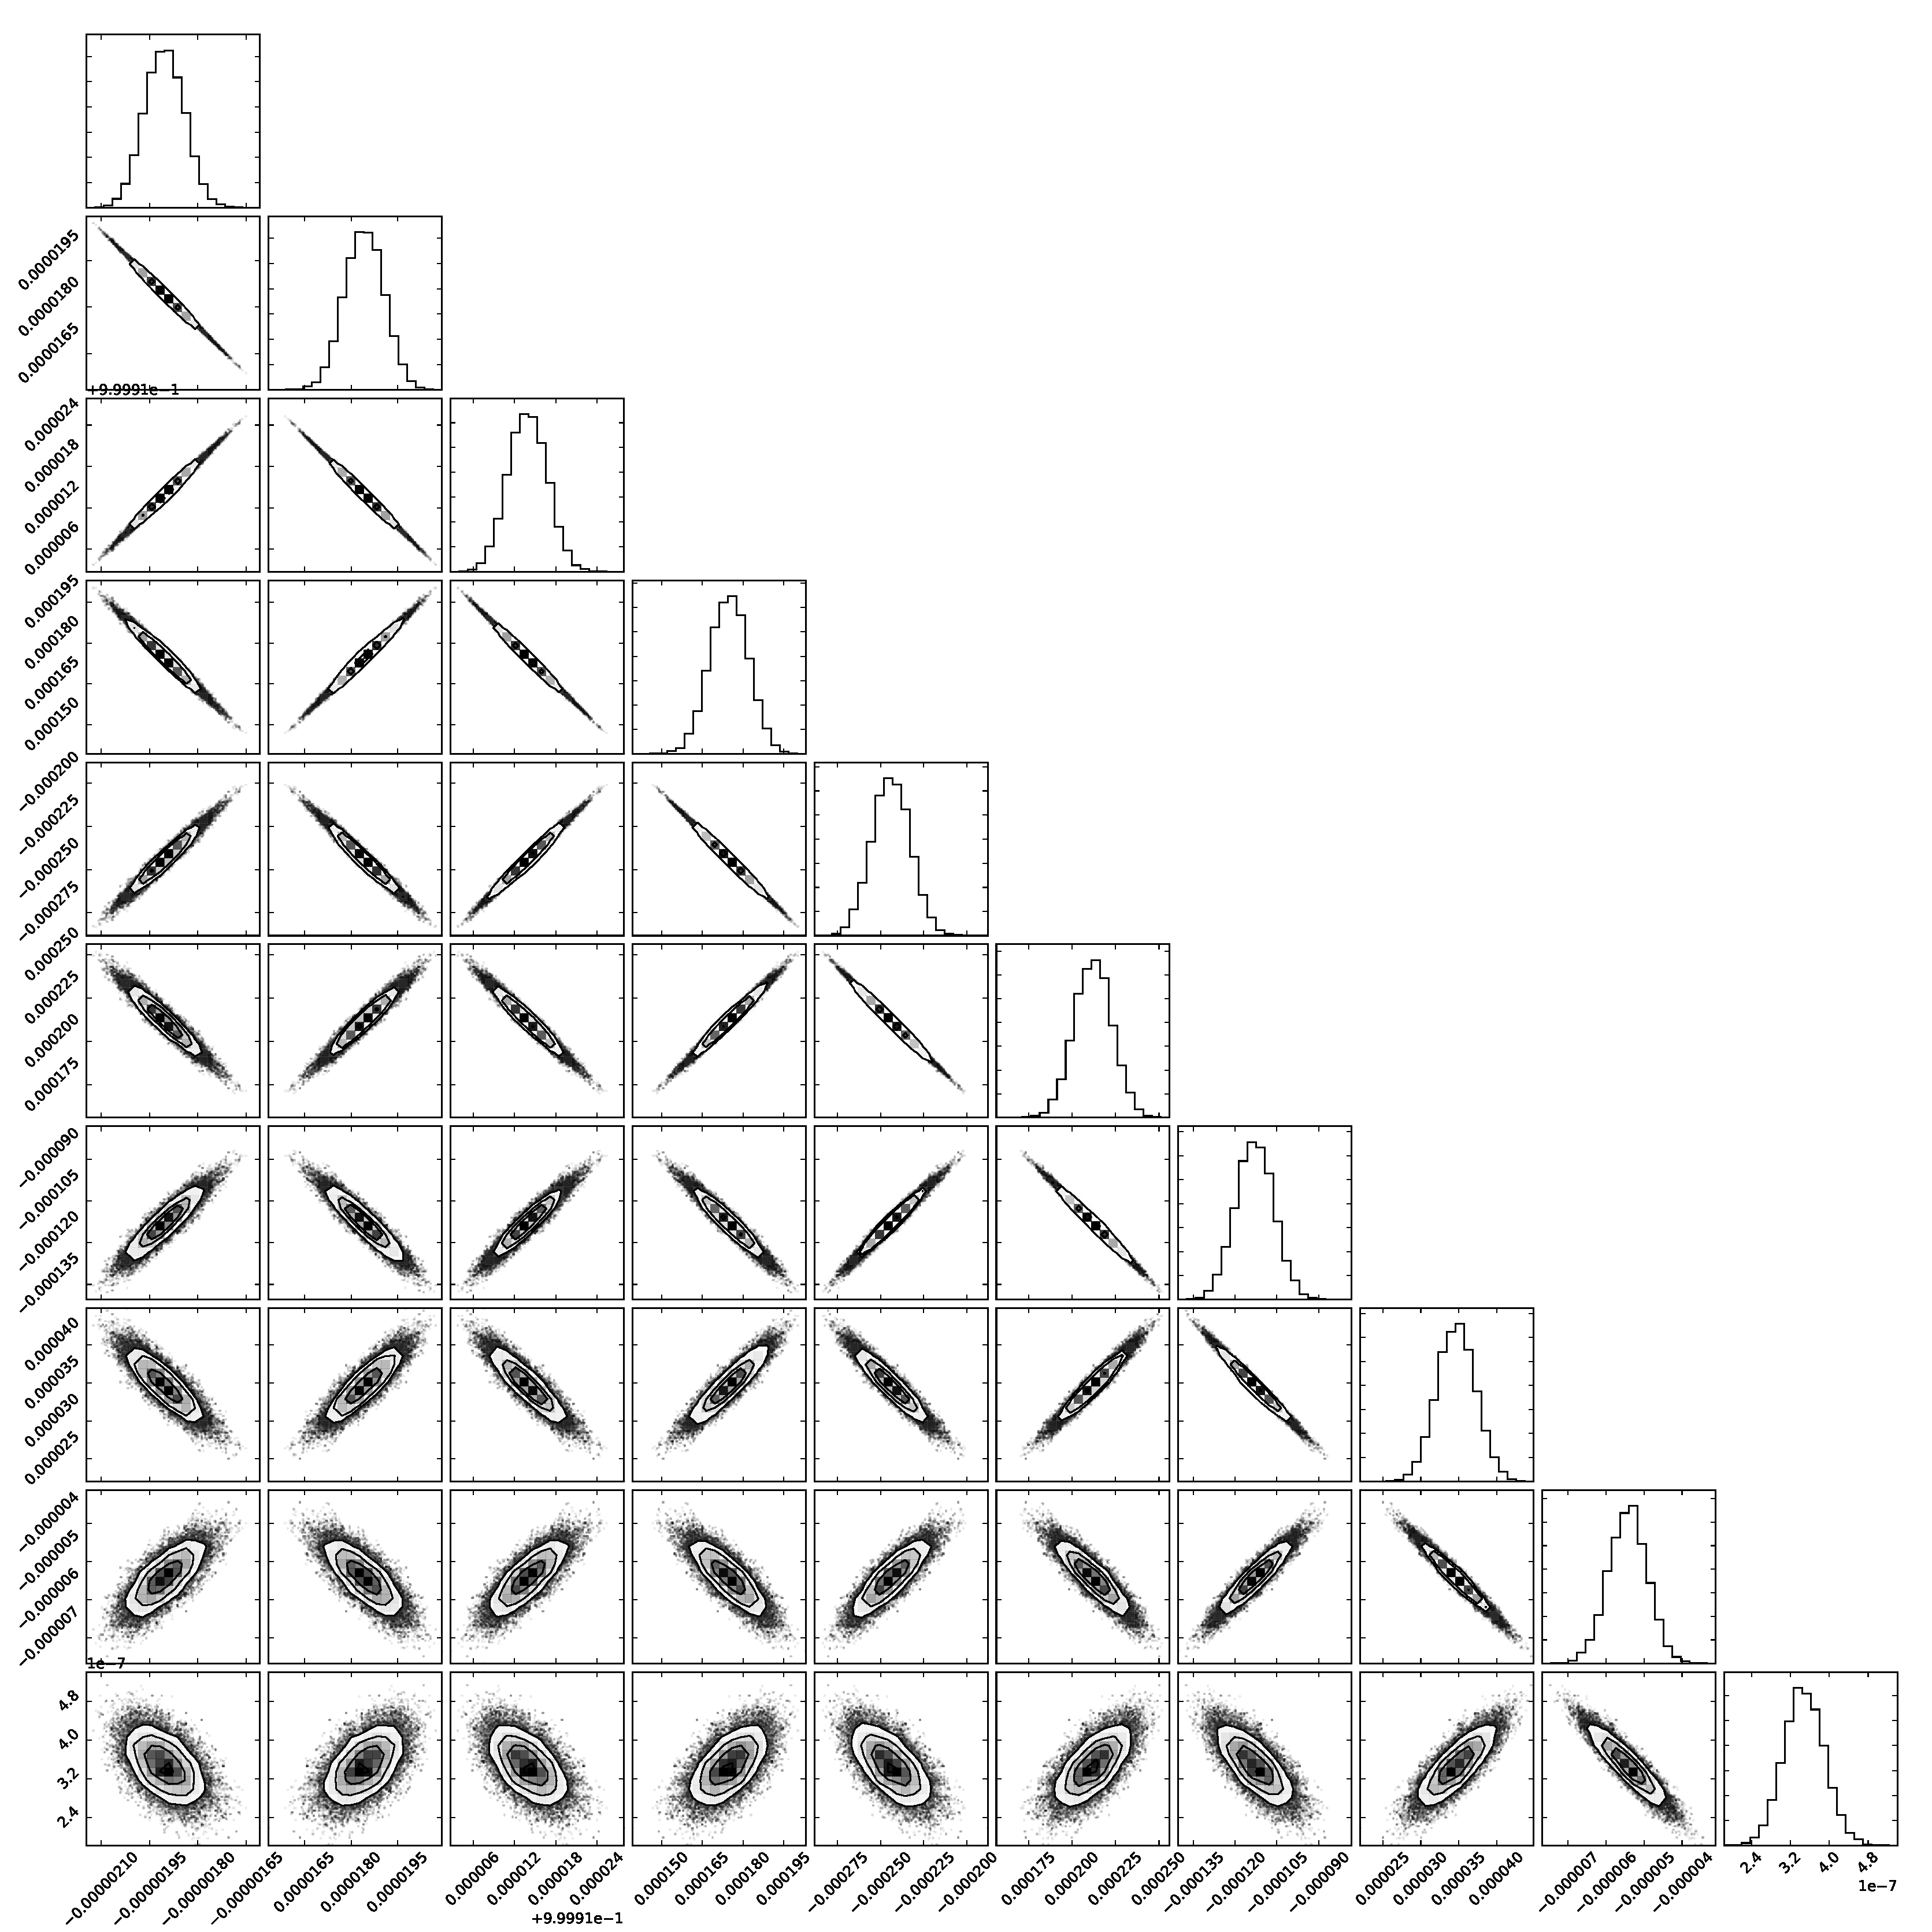
\includegraphics[width=\textwidth]{img/line-triangle.pdf}
  \caption{Corner plot of MCMC fit coefficients.}
  \label{fig:MCMC_triangle}
\end{figure*}

